% ======================================================================
% ARTIGO CIENTÍFICO-TECNOLÓGICO — ESPECIAÇÃO DE MERCÚRIO (Automação e IHM)
% Classe: article. Compilar: pdflatex -> bibtex -> pdflatex -> pdflatex.
% ======================================================================
\documentclass[11pt,a4paper]{article}

\usepackage[utf8]{inputenc}
\usepackage[T1]{fontenc}
\usepackage[brazilian]{babel}
\shorthandoff{"}                 % desativa shorthand " do babel brazilian
\usepackage{mathptmx}            % fonte Times
\usepackage[margin=2.5cm]{geometry}
\setlength{\emergencystretch}{3em} % reduz linhas "overfull" sem afetar a justificação
\usepackage{amsmath,amssymb}
\usepackage{graphicx}
\graphicspath{{figures/}}
\usepackage{booktabs}
\usepackage{float}
\usepackage{caption}
\usepackage[numbers,sort&compress]{natbib}
\usepackage{hyperref}
\usepackage{tikz}
\usetikzlibrary{arrows.meta,positioning}

\newcommand{\celsius}{\ensuremath{^{\circ}\mathrm{C}}}
\newcommand{\daq}{DAQ}

\title{Automa\c{c}\~ao e supervis\~ao da prepara\c{c}\~ao de amostras para
especia\c{c}\~ao de merc\'urio: arquitetura mestre-escravo com Raspberry Pi,
Arduino e IHM Web}

\author{
William da Silva Vianna \\
\small Instituto Federal Fluminense (IFF) --- Campos dos Goytacazes, RJ, Brasil
\\[1.2em]
Renato Gomes Sobral Barcellos \\
\small Instituto Federal Fluminense (IFF) --- Campos dos Goytacazes, RJ, Brasil
}
\date{}

\begin{document}

\maketitle

\begin{abstract}
\noindent A especia\c{c}\~ao de merc\'urio exige o controle rigoroso de uma
sequ\^encia de prepara\c{c}\~ao de amostras --- deriva\c{c}\~ao com
tetraetilborato de s\'odio, criofocaliza\c{c}\~ao em nitrog\^enio l\'iquido e
libera\c{c}\~ao t\'ermica controlada ---, em que a qualidade da rampa de
temperatura imposta ao Tubo U determina a correta separa\c{c}\~ao das esp\'ecies.
Este artigo apresenta o projeto e a valida\c{c}\~ao de um sistema de automa\c{c}\~ao
e supervis\~ao concebido para modernizar um sistema legado baseado em LabVIEW,
adotando uma arquitetura mestre-escravo formada por um Raspberry Pi (l\'ogica de
alto n\'ivel em Python), um Arduino Uno como m\'odulo de aquisi\c{c}\~ao de dados
em tempo real e uma interface homem-m\'aquina (IHM) Web em React e TypeScript. O
processo \'e modelado como uma m\'aquina de estados finita com quatro fases de
acionamento e matriz de atuadores; o controle de temperatura combina uma
estrat\'egia PID mista (raz\~ao de taxas abaixo de $0\,\celsius$ e PID em malha
fechada acima) para a rampa do Tubo U e um controle em setpoint fixo de
$700\,\celsius$ para o Forno 2. A comunica\c{c}\~ao entre as plataformas \'e feita
por pacotes JSON em enlace serial a 4~Hz, com watchdog duplo que imp\~oe o retorno
ao estado seguro em caso de falha. A valida\c{c}\~ao, conduzida por
desenvolvimento orientado a testes, resultou em 67 testes automatizados
aprovados distribu\'idos entre backend, firmware e IHM Web, evidenciando a
viabilidade da arquitetura para atender aos requisitos funcionais e de
seguran\c{c}a definidos. A valida\c{c}\~ao experimental em bancada com o processo
f\'isico permanece como etapa de continuidade.
\end{abstract}

\vspace{0.5em}
\noindent\textbf{Palavras-chave:} automa\c{c}\~ao; controle PID; especia\c{c}\~ao
de merc\'urio; m\'aquina de estados finita; sistemas embarcados; interface
homem-m\'aquina.

% ======================================================================
% SEÇÃO 1 — INTRODUÇÃO
% ======================================================================
\section{Introdu\c{c}\~ao}
\label{sec:intro}

O merc\'urio (Hg) \'e um poluente global cuja toxicidade e mobilidade dependem
fortemente da esp\'ecie qu\'imica em que se encontra. A \emph{especia\c{c}\~ao}
de merc\'urio --- a determina\c{c}\~ao das diferentes formas do elemento em uma
amostra --- \'e, portanto, essencial para avalia\c{c}\~oes de risco e estudos
biogeoqu\'imicos \cite{leermakers2005}. No sistema considerado neste trabalho,
a etapa de \emph{prepara\c{c}\~ao de amostras} compreende uma sequ\^encia
qu\'imica rigorosa: a amostra \'e derivatizada com tetraetilborato de s\'odio
(TEBS), volatilizando as esp\'ecies de merc\'urio; um g\'as de arraste (h\'elio)
conduz os vapores at\'e um Tubo U imerso em nitrog\^enio l\'iquido, onde ocorre a
\emph{criofocaliza\c{c}\~ao} a aproximadamente $-196\,\celsius$; em seguida, o
Tubo U \'e aquecido em uma rampa de temperatura e as esp\'ecies s\~ao liberadas
progressivamente conforme sua volatilidade, atomizadas a $700\,\celsius$ e
detectadas por espectrometria de absor\c{c}\~ao at\^omica
\cite{bloom1989,liang1994,lumex}.

A qualidade anal\'itica desse processo depende diretamente da
\emph{linearidade da rampa de temperatura} imposta ao Tubo U: desvios na rampa
provocam picos sobrepostos e an\'alises inv\'alidas. O equipamento originalmente
empregado era controlado por um sistema supervis\'orio legado desenvolvido em
LabVIEW, que apresentava limita\c{c}\~oes relevantes: (i) controle inadequado da
rampa, sem garantir a linearidade na faixa de $-50\,\celsius$ a
$230\,\celsius$; (ii) par\^ametros n\~ao persistentes e pouco rastre\'aveis entre
execu\c{c}\~oes; (iii) interface propensa a erro humano; (iv) acoplamento entre a
l\'ogica de aplica\c{c}\~ao e a execu\c{c}\~ao em tempo real; e (v) aus\^encia de
parada segura autom\'atica diante de falhas de comunica\c{c}\~ao.

Apesar da vasta literatura sobre m\'etodos de especia\c{c}\~ao
\cite{bloom1989,liang1994,leermakers2005} e sobre controle de temperatura com
controladores PID \cite{astrom2006,ogata2010}, h\'a uma lacuna no dom\'inio
considerado: a disponibilidade de uma solu\c{c}\~ao aberta e de baixo custo que
integre o sequenciamento da prepara\c{c}\~ao de amostras, o controle da rampa do
Tubo U e uma IHM moderna com persist\^encia de par\^ametros e seguran\c{c}a
funcional, em substitui\c{c}\~ao a plataformas propriet\'arias monol\'iticas.
Nesse contexto, este artigo tem como objetivo apresentar o projeto, a
implementa\c{c}\~ao e a valida\c{c}\~ao de um sistema de automa\c{c}\~ao e
supervis\~ao para a prepara\c{c}\~ao de amostras em especia\c{c}\~ao de
merc\'urio, baseado em uma arquitetura mestre-escravo composta por Raspberry Pi,
Arduino Uno e IHM Web.

A contribui\c{c}\~ao principal \'e a integra\c{c}\~ao coesa e verific\'avel de:
(i) uma m\'aquina de estados finita com matriz de acionamento dos atuadores;
(ii) uma estrat\'egia de controle PID mista que contorna a limita\c{c}\~ao de
medi\c{c}\~ao do termopar na regi\~ao criog\^enica; (iii) um protocolo JSON
aberto a 4~Hz; e (iv) mecanismos expl\'icitos de seguran\c{c}a (estado seguro e
watchdog duplo). O artigo est\'a organizado da seguinte forma: a Se\c{c}\~ao~2
apresenta a fundamenta\c{c}\~ao e os trabalhos relacionados; a Se\c{c}\~ao~3
descreve os materiais e m\'etodos, incluindo a arquitetura e a implementa\c{c}\~ao;
a Se\c{c}\~ao~4 apresenta os resultados da valida\c{c}\~ao; a Se\c{c}\~ao~5
discute os resultados e as limita\c{c}\~oes; e a Se\c{c}\~ao~6 conclui o artigo.

% ======================================================================
% SEÇÃO 2 — FUNDAMENTAÇÃO E TRABALHOS RELACIONADOS
% ======================================================================
\section{Fundamenta\c{c}\~ao e trabalhos relacionados}
\label{sec:fund}

\subsection{Especia\c{c}\~ao de merc\'urio e instrumenta\c{c}\~ao anal\'itica}

A determina\c{c}\~ao de esp\'ecies de merc\'urio em concentra\c{c}\~oes tra\c{c}o
exige etapas de deriva\c{c}\~ao qu\'imica que convertam as esp\'ecies em formas
vol\'ateis e est\'aveis, adequadas \`a separa\c{c}\~ao e \`a detec\c{c}\~ao.
Bloom \cite{bloom1989} e Liang e colaboradores \cite{liang1994} estabeleceram os
protocolos de etila\c{c}\~ao em fase aquosa com NaBEt$_4$ e de separa\c{c}\~ao
por cromatografia gasosa com detec\c{c}\~ao por fluoresc\^encia at\^omica em vapor
frio, que s\~ao a base qu\'imica do processo aqui automatizado. Revis\~oes como a
de Leermakers e colaboradores \cite{leermakers2005} evidenciam que a
repetibilidade das condi\c{c}\~oes de prepara\c{c}\~ao --- em particular da rampa
t\'ermica --- \'e um fator cr\'itico de qualidade dos m\'etodos de
especia\c{c}\~ao. No plano instrumental, equipamentos comerciais dedicados, como
o analisador RA-915 da Lumex \cite{lumex}, integram a atomiza\c{c}\~ao e a
detec\c{c}\~ao, mas tipicamente n\~ao exp\~oem ao usu\'ario o controle fino do
sequenciamento da prepara\c{c}\~ao que antecede a medida --- refor\c{c}ando a
relev\^ancia de um sistema de automa\c{c}\~ao dedicado a essa etapa.

\subsection{Controle de processos e rampas de temperatura}

Em processos cuja vari\'avel controlada deve seguir uma trajet\'oria no tempo,
como a rampa linear de temperatura do Tubo U, o controlador
proporcional-integral-derivativo (PID) \'e a solu\c{c}\~ao mais difundida
\cite{astrom2006,ogata2010}. Em sua forma cont\'inua ideal, a sa\'ida \'e dada
por
\begin{equation}
  u(t) = K_p \left[ e(t) + \frac{1}{T_i}\int_0^t e(\tau)\,d\tau
         + T_d \frac{d\,e(t)}{dt} \right],
  \label{eq:pid}
\end{equation}
em que $K_p$ \'e o ganho proporcional, $T_i$ o tempo integral e $T_d$ o tempo
derivativo. Implementa\c{c}\~oes digitais devem tratar a satura\c{c}\~ao da sa\'ida
(anti-windup) e aplicar a a\c{c}\~ao derivativa sobre a vari\'avel de processo,
evitando o \emph{derivative kick} \cite{astrom2006}. Quando a medi\c{c}\~ao n\~ao
\'e confi\'avel em parte da faixa --- como abaixo do piso de leitura do termopar
---, uma estrat\'egia de raz\~ao de taxas em malha aberta pode ser combinada ao
PID, calculando a vari\'avel manipulada proporcionalmente \`a rela\c{c}\~ao entre
a taxa de aquecimento desejada e a taxa do sistema.

O controle sequencial de processos \'e frequentemente modelado por
\emph{m\'aquinas de estado finitas} (FSM), que associam a cada estado um conjunto
de sa\'idas ativas (matriz de acionamento) e tratam de forma sistem\'atica
eventos de parada e emerg\^encia \cite{wagner2006}.

\subsection{Plataformas embarcadas e comunica\c{c}\~ao}

A literatura e a pr\'atica de instrumenta\c{c}\~ao anal\'itica adotam, com
crescente frequ\^encia, plataformas abertas de baixo custo: microcontroladores
como o Arduino \cite{arduino} e computadores de placa \'unica como o Raspberry Pi
\cite{raspberrypi}. A separa\c{c}\~ao entre uma camada de supervis\~ao de alto
n\'ivel e um m\'odulo de aquisi\c{c}\~ao em tempo real melhora a confiabilidade e
a manutenibilidade. A medi\c{c}\~ao de temperatura por termopares tipo K \'e
comumente digitalizada por circuitos integrados com compensa\c{c}\~ao de
jun\c{c}\~ao fria, como o MAX6675, que entrega 12~bits com resolu\c{c}\~ao de
$0{,}25\,\celsius$ via SPI \cite{max6675,nist_its90}.

A comunica\c{c}\~ao entre plataformas \'e realizada com pacotes JSON
\cite{bray2017} em enlace serial, e a IHM Web consome uma API REST e telemetria
em tempo real via WebSocket \cite{fette2011}. Frameworks modernos como FastAPI
\cite{fastapi} e React \cite{react} permitem construir supervis\'orios acess\'iveis
por navegador, em contraste com plataformas propriet\'arias monol\'iticas
(frequentemente baseadas em LabVIEW) que acoplam controle, interface e
aquisi\c{c}\~ao em um \'unico ambiente, com custo elevado de licenciamento e
evolu\c{c}\~ao restrita.

\subsection{S\'intese e lacuna}

A revis\~ao indica que n\~ao h\'a, no dom\'inio considerado, uma solu\c{c}\~ao
aberta e de baixo custo que integre, de forma coesa e segura, o sequenciamento da
prepara\c{c}\~ao de amostras, o controle PID da rampa do Tubo U e uma IHM Web com
persist\^encia de par\^ametros. Este artigo busca preencher essa lacuna, com
\^enfase na rastreabilidade entre requisitos, implementa\c{c}\~ao e valida\c{c}\~ao
por testes.

% ======================================================================
% SEÇÃO 3 — MATERIAIS E MÉTODOS
% ======================================================================
\section{Materiais e m\'etodos}
\label{sec:met}

\subsection{Arquitetura do sistema}

O sistema adota uma topologia mestre-escravo. O \emph{mestre} \'e um Raspberry Pi
que executa o backend em Python: a m\'aquina de estados, os controladores, a
persist\^encia de par\^ametros, a API REST/WebSocket e o servi\c{c}o da IHM. O
\emph{escravo} \'e um Arduino Uno que opera como m\'odulo de aquisi\c{c}\~ao de
dados (\daq) em tempo real: aplica comandos de atuadores, gera os PWM dos fornos e
l\^e termopares via SPI. A comunica\c{c}\~ao entre as plataformas \'e feita por um
enlace serial USB com pacotes JSON em ciclo de 4~Hz. A Figura~\ref{fig:arq}
apresenta a arquitetura e o fluxo de dados.

\begin{figure}[htbp]
\centering
\begin{tikzpicture}[
  font=\small,
  box/.style={rectangle, draw, minimum width=3.2cm, minimum height=1.0cm,
              align=center, rounded corners=2pt},
  arr/.style={-{Latex[length=2mm]}, thick}
]
  \node[box] (ihm) at (0,2.4) {IHM Web\\ (React + TypeScript)};
  \node[box] (be)  at (0,0) {Backend (Raspberry Pi)\\ FSM + PID + persist\^encia};
  \node[box] (daq) at (0,-2.4) {\daq{} Arduino Uno\\ atuadores + SPI + watchdog};
  \node[box] (pr)  at (0,-4.6) {Processo f\'isico\\ v\'alvulas, bomba, fornos, termopares};
  \node[box, minimum width=3.2cm, minimum height=0.9cm] (st) at (6.4,0) {Par\^ametros\\ (JSON em disco)};
  \draw[arr,<->] (ihm) -- node[right]{HTTP/WS} (be);
  \draw[arr,<->] (be) -- node[right]{serial JSON 4~Hz} (daq);
  \draw[arr] (be) -- node[above]{escrita} (st);
  \draw[arr] (st) -- node[above]{leitura} (be);
  \draw[arr,<->] (daq) -- node[right]{sinais} (pr);
\end{tikzpicture}
\caption{Arquitetura mestre-escravo e fluxo de dados do sistema.}
\label{fig:arq}
\end{figure}

\subsection{Descri\c{c}\~ao do processo e modelagem}

O processo de prepara\c{c}\~ao foi modelado em uma FSM com os estados seguro
(\texttt{SAFE}), deriva\c{c}\~ao/\allowbreak criofocaliza\c{c}\~ao ($T_0$),
estabiliza\c{c}\~ao ($T_1$), rampa ($T_2$), purga total ($T_3$) e manual
(\texttt{MANUAL}). A cada estado associa-se uma matriz de acionamento das
sa\'idas discretas (v\'alvulas SV1 a SV5 e bomba perist\'altica), apresentada na
Tabela~\ref{tab:matriz}, em que 1 indica atuador acionado. Eventos de parada
(\texttt{stop}) e de emerg\^encia (\texttt{emergency}) podem ocorrer a qualquer
momento e conduzem ao estado seguro; o modo manual permite o acionamento direto
dos atuadores para manuten\c{c}\~ao.

\begin{table}[htbp]
\centering
\caption{Matriz de acionamento dos atuadores por fase do ciclo.}
\label{tab:matriz}
\begin{tabular}{lcccccc}
\toprule
\textbf{Fase} & \textbf{SV1} & \textbf{SV2} & \textbf{SV3} & \textbf{SV4} & \textbf{SV5} & \textbf{Bomba} \\
\midrule
$T_0$ (deriva\c{c}\~ao/criofocaliza\c{c}\~ao) & 1 & 0 & 0 & 0 & 1 & 1 \\
$T_1$ (estabiliza\c{c}\~ao) & 1 & 0 & 0 & 0 & 1 & 0 \\
$T_2$ (rampa/purga) & 1 & 0 & 0 & 0 & 0 & 0 \\
$T_3$ (purga total) & 0 & 1 & 1 & 1 & 0 & 0 \\
SAFE & 0 & 0 & 0 & 0 & 0 & 0 \\
\bottomrule
\end{tabular}
\end{table}

\subsection{Controle de temperatura}

O controle de temperatura emprega uma estrat\'egia PID mista, implementada no
backend e detalhada a seguir.

\textbf{Forno 2 (atomizador):} opera em malha fechada com setpoint fixo de
$700\,\celsius$ durante as fases $T_0$ a $T_2$, com controlador discreto P+I,
anti-windup por clampagem e deriva\c{c}\~ao sobre a vari\'avel de processo. Os
ganhos padr\~ao s\~ao $K_p = 44{,}67$, $T_i = 0{,}18$~min e $T_d = 0$.

\textbf{Forno 1 (Tubo U):} combina duas regi\~oes de controle, selecionadas pela
temperatura medida $T_1$:
\begin{itemize}
  \item \textbf{$T_1 < 0\,\celsius$:} a medi\c{c}\~ao n\~ao \'e confi\'avel; a
  vari\'avel manipulada \'e calculada em malha aberta pela raz\~ao de taxas
  \begin{equation}
    VM = \frac{\dot{T}_{\mathrm{des}}}{\dot{T}_{\mathrm{sist}}} \times VM_{\max},
    \label{eq:razao}
  \end{equation}
  em que $\dot{T}_{\mathrm{des}}$ \'e a taxa de aquecimento desejada pelo
  operador, $\dot{T}_{\mathrm{sist}}$ a taxa do sistema (calibrada em bancada) e
  $VM_{\max}=255$ o valor m\'aximo da sa\'ida PWM;
  \item \textbf{$T_1 \ge 0\,\celsius$:} um PID em malha fechada segue o setpoint
  din\^amico da rampa, $r(t)=T_{N_2}+\dot{T}_{\mathrm{des}}\,t$, limitado ao alvo
  de $230\,\celsius$, em que $T_{N_2}$ \'e a temperatura inicial do nitrog\^enio.
\end{itemize}

A taxa de aquecimento desejada \'e calculada por
$\dot{T}_{\mathrm{des}}=(T_{\mathrm{alvo}}-T_{N_2})/t_{\mathrm{rampa}}$ e \'e o
coeficiente exibido na IHM, em $^{\circ}$C/s.

\subsection{Implementa\c{c}\~ao}

O backend (\texttt{Python} + FastAPI \cite{fastapi}) \'e organizado em m\'odulos
de FSM, controlador PID, rampa, enlace serial, loop de controle, persist\^encia e
API. O loop de controle roda em uma thread dedicada a 4~Hz: a cada itera\c{c}\~ao
envia o pacote de escrita ao \daq, l\^e a resposta (temperaturas e estado),
atualiza a FSM e publica a telemetria. O \emph{watchdog do backend} comuta a FSM
para o estado seguro se n\~ao houver resposta do \daq por mais de 1~s.

O firmware do Arduino \'e organizado em c\'odigo de aplica\c{c}\~ao e em uma
biblioteca port\'avel (\texttt{daqcore}) contendo o parser JSON, o watchdog e a
l\'ogica de pulso da bomba. O firmware l\^e termopares via SPI (12~bits, LSB
$0{,}25\,\celsius$), mantendo o \'ultimo valor v\'alido durante convers\~ao ou
falha transit\'oria, e aplica os atuadores; o \emph{watchdog do firmware} desliga
os fornos se nenhum pacote v\'alido for recebido em mais de 1~s. A bomba
perist\'altica possui comportamento de trava por pulso: o firmware detecta a
transi\c{c}\~ao do estado l\'ogico e emite um pulso de $600$~ms que alterna o
estado f\'isico da bomba.

Os par\^ametros do m\'etodo (ganhos PID, tempos $t_1$, $t_2$, $t_3$, rampa,
temperatura do nitrog\^enio, temperatura alvo e setpoint do Forno 2) s\~ao
persistidos em arquivo JSON no Raspberry Pi com escrita at\^omica e backup
rotativo, assegurando integridade e auditoria.

A IHM Web (\texttt{React} + TypeScript \cite{react}) \'e servida pelo pr\'oprio
backend e organizada em modos de monitoramento e de configura\c{c}\~ao,
incluindo um Diagrama de Tempos das fases $T_0$ a $T_3$, painel de controles e
atuadores, gr\'aficos de tend\^encia por forno e formul\'ario de configura\c{c}\~ao
do m\'etodo, consumindo a API REST e o WebSocket de telemetria \cite{fette2011}.

\subsection{Ambiente e procedimento de valida\c{c}\~ao}

A valida\c{c}\~ao foi conduzida em ambiente de desenvolvimento, sem o hardware
f\'isico do processo, seguindo desenvolvimento orientado a testes
\cite{beck2002}. Tr\^es frentes foram executadas:

\begin{itemize}
  \item \textbf{Backend (Python):} testes unit\'arios (FSM, PID, rampa,
  persist\^encia, enlace serial), testes da API e testes funcionais de ciclo
  completo e de seguran\c{c}a, com \texttt{pytest};
  \item \textbf{Firmware:} testes \emph{host-based} da biblioteca \texttt{daqcore}
  (parser JSON, watchdog e pulso da bomba) no ambiente \texttt{native} do
  PlatformIO;
  \item \textbf{IHM Web:} testes unit\'arios dos \emph{stores} de telemetria,
  acionamento manual e tema, com Vitest.
\end{itemize}

Os testes funcionais e de seguran\c{c}a utilizam um simulador do \daq conectado
ao backend por portas seriais virtuais criadas com \texttt{socat}, permitindo
exercitar o ciclo $T_0 \to T_3$ e simular a perda de comunica\c{c}\~ao sem
hardware. A Tabela~\ref{tab:criterios} consolida os crit\'erios de aceita\c{c}\~ao.

\begin{table}[htbp]
\centering
\caption{Crit\'erios de aceita\c{c}\~ao da valida\c{c}\~ao.}
\label{tab:criterios}
\begin{tabular}{p{4.6cm}p{4.6cm}p{5.6cm}}
\toprule
\textbf{M\'etrica} & \textbf{Alvo} & \textbf{Forma de medi\c{c}\~ao} \\
\midrule
Linearidade da rampa (Tubo U) & Desvio $\le \pm 2\,\celsius$ do SP & Curva VP$\times$SP em bancada \\
Estabilidade do Forno 2 & $\pm 5\,\celsius$ em torno de $700\,\celsius$ & Curva VP$\times$SP em bancada \\
Comunica\c{c}\~ao a 4~Hz & 100\% em 4~h de estresse & Teste de estresse integrado \\
Persist\^encia de par\^ametros & 100\% \'integra ap\'os rein\'icio & Teste funcional \\
Seguran\c{c}a (watchdog) & Fornos desligados em $\le 1$~s & Teste de perda de serial \\
\bottomrule
\end{tabular}
\end{table}

% ======================================================================
% SEÇÃO 4 — RESULTADOS
% ======================================================================
\section{Resultados}
\label{sec:res}

Os resultados reportados correspondem a execu\c{c}\~oes reais das su\'ites de
testes automatizados realizadas no ambiente de desenvolvimento do projeto. A
Tabela~\ref{tab:testes} consolida os resultados por camada.

\begin{table}[htbp]
\centering
\caption{Resultado da execu\c{c}\~ao das su\'ites de testes automatizados.}
\label{tab:testes}
\begin{tabular}{lcccc}
\toprule
\textbf{Camada} & \textbf{Ferramenta} & \textbf{Arquivos} & \textbf{Testes} & \textbf{Resultado} \\
\midrule
Backend (Python) & pytest & 8 & 40 & 40 aprovados \\
Firmware (\daq) & PlatformIO (host) & 1 & 14 & 14 aprovados \\
IHM Web & Vitest & 4 & 13 & 13 aprovados \\
\midrule
\textbf{Total} & --- & 13 & 67 & 67 aprovados \\
\bottomrule
\end{tabular}
\end{table}

\subsection{Testes de l\'ogica e integra\c{c}\~ao}

Os testes do backend validaram as transi\c{c}\~oes da FSM e a matriz de
acionamento em cada fase; o c\'alculo da sa\'ida do PID, a satura\c{c}\~ao e o
anti-windup; o c\'alculo da taxa de aquecimento e a sele\c{c}\~ao das duas
regi\~oes da rampa (raz\~ao de taxas abaixo de $0\,\celsius$ e PID acima); a
escrita/leitura at\^omicas da persist\^encia com restaura\c{c}\~ao do backup; o
codec JSON do enlace serial; e os endpoints da API. Os testes do firmware
validaram o parser de pacotes JSON, a rejei\c{c}\~ao de JSON inv\'alido, a
constru\c{c}\~ao do pacote de resposta, o watchdog (disparo, rearme e
configura\c{c}\~ao do tempo limite) e o pulso de toggle da bomba. Os testes do
frontend validaram o consumo da telemetria WebSocket, o sincronismo dos controles
manuais com a telemetria e a persist\^encia da prefer\^encia de tema.

\subsection{Testes funcionais e de seguran\c{c}a}

Os testes funcionais exercitaram o ciclo autom\'atico $T_0 \to T_3$ com o
simulador do \daq, confirmando que: (i) o ciclo somente inicia a partir do estado
seguro; (ii) as dura\c{c}\~oes das fases seguem os par\^ametros configurados; e
(iii) a telemetria publicada cont\'em o estado, o progresso da etapa e o
progresso geral do ciclo, habilitando o Diagrama de Tempos da IHM. Os cen\'arios
de seguran\c{c}a simularam a perda de comunica\c{c}\~ao serial e confirmaram as
duas camadas de prote\c{c}\~ao: o watchdog do firmware desliga os fornos na
aus\^encia de pacotes v\'alidos por mais de 1~s, e o watchdog do backend comuta a
FSM para o estado seguro quando o \daq deixa de responder por mais de 1~s,
atendendo ao crit\'erio de fornos desligados em $\le 1$~s.

A Figura~\ref{fig:ihm} apresenta a IHM Web em opera\c{c}\~ao, exibindo o Diagrama
de Tempos, o progresso da etapa, os controles e atuadores e os gr\'aficos de
tend\^encia por forno.

\begin{figure}[htbp]
\centering
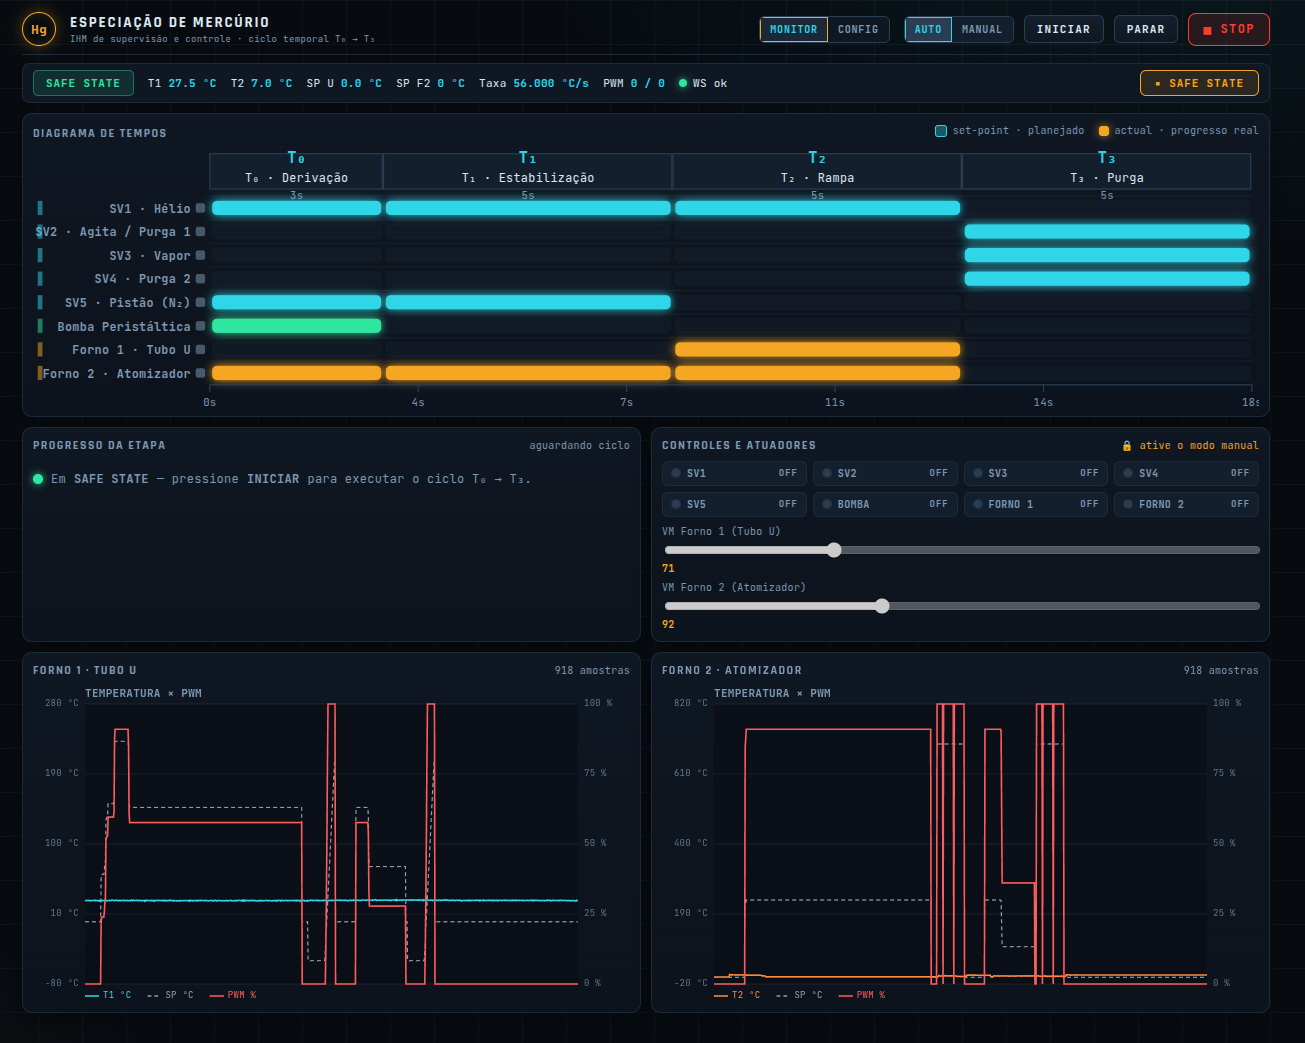
\includegraphics[width=0.9\linewidth]{frontendweb.png}
\caption{IHM Web em modo de monitoramento.}
\label{fig:ihm}
\par\vspace{2pt}{\footnotesize Fonte: captura de tela da IHM do projeto.}
\end{figure}

% ======================================================================
% SEÇÃO 5 — DISCUSSÃO
% ======================================================================
\section{Discuss\~ao}
\label{sec:disc}

Os resultados indicam que a implementa\c{c}\~ao atende aos objetivos funcionais e
de seguran\c{c}a definidos, com 67 testes aprovados distribu\'idos pelas tr\^es
camadas do sistema. Tr\^es observa\c{c}\~oes merecem destaque. Primeiro, os testes
de FSM, PID e rampa validam matematicamente a estrat\'egia de controle mista,
incluindo o tratamento da satura\c{c}\~ao e a sele\c{c}\~ao da regi\~ao de
opera\c{c}\~ao --- condi\c{c}\~ao necess\'aria, ainda que n\~ao suficiente, para a
qualidade da rampa em bancada. Segundo, a valida\c{c}\~ao dos watchdogs em ambas
as camadas demonstra que o requisito de parada segura autom\'atica \'e atendido no
n\'ivel de software, independentemente do hardware. Terceiro, os testes de ciclo
completo com simulador confirmam a coer\^encia entre a FSM, o protocolo serial e a
telemetria consumida pela IHM, reduzindo o risco de falhas de integra\c{c}\~ao
quando o hardware real for conectado.

Dos crit\'erios de aceita\c{c}\~ao consolidados na Tabela~\ref{tab:criterios},
tr\^es foram verific\'aveis no ambiente simulado (comunica\c{c}\~ao a 4~Hz,
persist\^encia e watchdog) e dois dependem de medi\c{c}\~ao em bancada
(linearidade da rampa e estabilidade do Forno 2). Esses \'ultimos s\~ao
crit\'erios de \emph{desempenho t\'ermico} do processo f\'isico e n\~ao podem ser
atestados por testes de software: exigem a calibra\c{c}\~ao da curva de
aquecimento do Tubo U (Taxa $\times$ PWM) e a verifica\c{c}\~ao experimental das
curvas de temperatura, etapas de continuidade deste trabalho.

A principal limita\c{c}\~ao \'e, portanto, a aus\^encia de medi\c{c}\~oes em
bancada com o processo f\'isico. Al\'em disso, a raz\~ao de taxas empregada na
regi\~ao de malha aberta depende da calibra\c{c}\~ao da taxa de aquecimento do
sistema; na aus\^encia desse dado, a implementa\c{c}\~ao adota uma aproxima\c{c}\~ao
que precisa ser confirmada. Registra-se, ainda, a indefini\c{c}\~ao quanto ao
circuito integrado exato de convers\~ao do termopar (MAX6675 ou MAX31855), que
n\~ao altera a l\'ogica de controle, mas deve ser confirmada na documenta\c{c}\~ao
f\'isica do equipamento.

No plano t\'ecnico, os resultados demonstram a viabilidade da arquitetura
proposta para substituir o sistema legado, com vantagens de custo, flexibilidade
e seguran\c{c}a. No plano operacional, a persist\^encia dos par\^ametros e o
registro de tend\^encias criam condi\c{c}\~oes para a repetibilidade e a auditoria
do m\'etodo, requisitos valorizados em ambiente anal\'itico. A etapa de
valida\c{c}\~ao em bancada \'e o passo natural para confirmar os crit\'erios de
desempenho t\'ermico e calibrar a rampa do Tubo U.

% ======================================================================
% SEÇÃO 6 — CONCLUSÃO
% ======================================================================
\section{Conclus\~ao}
\label{sec:concl}

Este artigo apresentou o projeto, a implementa\c{c}\~ao e a valida\c{c}\~ao de um
sistema de automa\c{c}\~ao e supervis\~ao para a prepara\c{c}\~ao de amostras em
especia\c{c}\~ao de merc\'urio, concebido para substituir um sistema legado
baseado em LabVIEW. A solu\c{c}\~ao adota uma arquitetura mestre-escravo composta
por um Raspberry Pi (l\'ogica de alto n\'ivel em Python), um Arduino Uno
(aquisi\c{c}\~ao em tempo real) e uma IHM Web em React e TypeScript, integrados por
um protocolo JSON a 4~Hz.

O objetivo proposto foi atingido no \^ambito da valida\c{c}\~ao realizada: o
processo foi modelado em uma m\'aquina de estados finita com matriz de
acionamento; o controle PID misto da rampa do Tubo U e o controle do Forno 2 a
$700\,\celsius$ foram implementados e verificados por testes; o protocolo JSON, o
firmware do \daq (leitura SPI, atuadores e watchdog), a persist\^encia at\^omica
dos par\^ametros e a IHM Web foram desenvolvidos e integrados. A valida\c{c}\~ao
por 67 testes automatizados aprovados demonstrou a corre\c{c}\~ao da l\'ogica de
controle, a integra\c{c}\~ao entre as camadas e a efetividade dos mecanismos de
seguran\c{c}a no n\'ivel de software.

As principais contribui\c{c}\~oes s\~ao: a modelagem expl\'icita e verific\'avel do
sequenciamento; a estrat\'egia de controle mista que contorna a limita\c{c}\~ao de
medi\c{c}\~ao na regi\~ao criog\^enica; a arquitetura mestre-escravo de baixo
custo com separa\c{c}\~ao entre supervis\~ao e tempo real; o protocolo JSON aberto;
e o projeto de seguran\c{c}a em camadas (estado seguro por padr\~ao e watchdog
duplo).

Como limita\c{c}\~ao, a valida\c{c}\~ao foi conduzida em ambiente simulado, sem o
processo f\'isico; os crit\'erios de desempenho t\'ermico e a calibra\c{c}\~ao da
curva de aquecimento do Tubo U permanecem pendentes de verifica\c{c}\~ao
experimental. Como trabalhos futuros, sugere-se: validar o sistema em bancada;
integrar automaticamente o detector Lumex e exportar as curvas geradas;
implementar autentica\c{c}\~ao de operadores com trilha de auditoria;
desenvolver um simulador de processo para treinamento; e implementar a
sintoniza\c{c}\~ao autom\'atica dos controladores PID.


\section*{Agradecimentos}
\textit{[Agradecimentos opcionais --- a redigir pelos autores (ex.: \`a
institui\c{c}\~ao e ao laborat\'orio).]}

\bibliographystyle{plain}
\bibliography{references}

\end{document}
